\documentclass{beamer}
\usetheme{Antibes}

% removes navigation icons
\setbeamertemplate{navigation symbols}{}

\usepackage[utf8]{inputenc}
\usepackage{hyperref}
\usepackage{framed}
\usepackage{graphicx}
\usepackage{color}
\usepackage{cite}


\newcommand{\remove}[1]{}
%\newcomand{\mynote}[1]{}

\title{Identificação de elementos em documentos HTML baseado em estruturas semelhantes}
\author[Iam Jabour]{Iam Jabour \\ Orientador: Eduardo Laber \\ Co-orientador: Raúl Rentería}
\institute[PUC-Rio]{
  Pontifícia Universidade Católica do Rio de Janeiro \\
}
\date{27 de Janeiro 2010}

\newenvironment{my_itemize}{
\begin{itemize}
  \setlength{\itemsep}{5pt}
  \setlength{\parskip}{2pt}
  \setlength{\parsep}{3pt}
}{\end{itemize}}


\begin{document}

\begin{frame}
  \titlepage
\end{frame}

\AtBeginSection[]{
  \begin{frame}
    \frametitle{Sumário}

    \tableofcontents[currentsection]
  \end{frame}
}


\section{Introdução}
\begin{frame}
  \subsection{Problema}
  \frametitle{Problema}
  \begin{my_itemize}
   \item Identificar e extrair conteúdo de documentos HTML

   \item Tarefas
   \begin{my_itemize}
    \item[-] Identificação de \textit{templates}: limpar o documento para diminuir a quantidade de informação não relevante 

    \item[-] \alert{Extração de tabelas: entender as informações apresentadas em tabelas}

    \item[-] Identificação de estruturas tabulares (tabelas, listas): identificar informações dispostas de forma estruturada 

    \item[-] \alert{Extração de itens em sites de comércio eletrônico: facilitar a recuperação de informação de itens}
    \end{my_itemize}

  \end{my_itemize}
\end{frame}

\begin{frame}[allowframebreaks]
  \subsection{Motivação}
  \frametitle{Motivação}
  \begin{my_itemize}
   \item Motivação geral
 
  \begin{my_itemize}
    \item Estudar documentos HTML em busca de padrões e estruturas que ajudem na resolução de tarefas de extração de conteúdo

    \item Apresentar resultados para a tarefa de identificação de tabelas genuínas, utilizando algoritmos com menor custo computacional

    \item Apresentar resultados para a tarefa de extração de itens em sites de comércio eletrônico

    \item Otimizar o tempo de processamento por documento
  \end{my_itemize}

   \item Motivação das Tarefas

   \begin{my_itemize}
    \item facilitar tarefas de recuperação de informação
   \end{my_itemize}

\end{my_itemize} 
\end{frame}

\begin{frame}[allowframebreaks]
  \subsection{Abordagem proposta}
  \frametitle{Abordagem proposta}
  \begin{my_itemize}
    \item Analisar a estrutura da árvore HTML em busca de semelhanças estruturais

    \item Agrupar o conjunto de informações que aparece com estrutura semelhante

\newpage
\begin{figure}[h]
    \includegraphics[scale=0.25]{img/tree0}
    \caption{Árvore HTML, sub-árvores vermelhas têm a mesma estrutura}
\end{figure}
\newpage
\begin{figure}[h]
    \includegraphics[scale=0.25]{img/tree1}
    \caption{Árvore que apresenta a mesma sub-estrutura, tipicamente listas e tabelas}
\end{figure}
\newpage
\begin{figure}[h]
    \includegraphics[scale=0.25]{img/tree2}
    \caption{Árvore que apresenta sub-estrutura semelhante}
\end{figure}
\newpage
\begin{figure}[h]
    \includegraphics[scale=0.25]{img/tree3}
    \caption{Árvore que não contem semelhança em sua estrutura}
\end{figure}
  \end{my_itemize}
\end{frame}


\section{Tarefas}
\begin{frame}[allowframebreaks]
  \subsection{Identificação de tabela genuína}
  \frametitle{Identificação de tabela genuína}
  \begin{my_itemize}
    \item Definição
    \begin{my_itemize}
    \item Tabela genuína: apresenta informações de forma tabular, onde o conteúdo de uma linha ou coluna tem o mesmo significado
    \end{my_itemize}

\begin{figure}[h]
    \center
    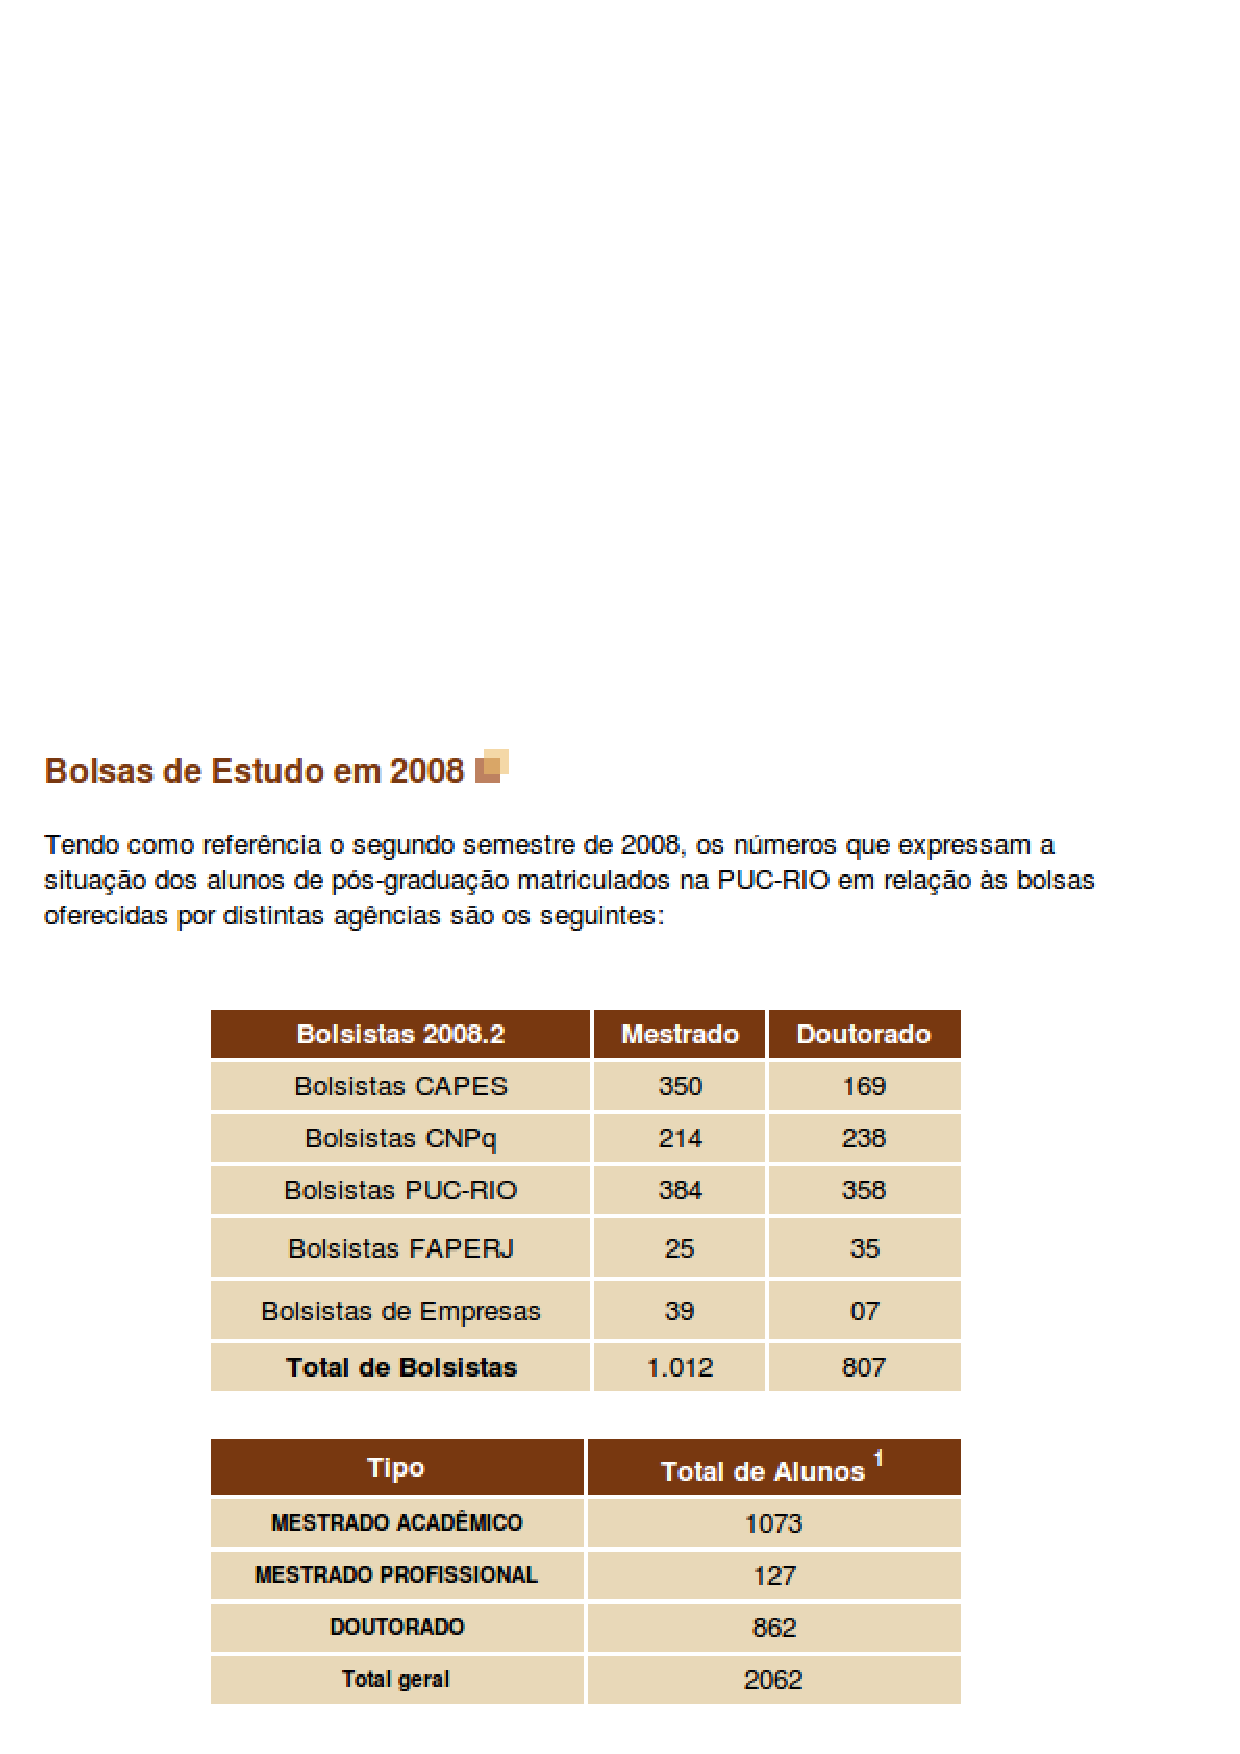
\includegraphics[scale=0.25]{img/table}
    \caption{retirado de: www.puc-rio.br/ensinopesq/ccpg/bolsas/html}
\end{figure}

\newpage
    \item ~\cite{Pinto2003} define 5 níveis de problemas na tarefa de extração de tabelas:
    \begin{my_itemize}
    \item[1] \alert{Localizar a tabela}
    \item[2] Identificar a posição das linhas e seus tipos
    \item[3] Identificar a posição das colunas e seus tipos
    \item[4] Tag the cells as data or headers
    \item[5] Associate data cells with their corresponding headers
    \end{my_itemize}

\newpage
    \item Motivação
    \begin{my_itemize}
    \item Importância de dados apresentados em tabelas
    \item Uso errado da \textit{tag} table por programadores
    \end{my_itemize}

    \item {\color{yellow}Trabalhos Relacionados}
    \begin{my_itemize}
    \item[-] ~\cite{Pinto2003}: Aborda o problema em texto puro, modela de forma a poder utilizar um Conditional Random Fields para resolver o problema de identificar linhas e determinar seus tipos.

   \item[-] ~\cite{Krupl2006}: Aborda o problema de forma visual, procurando blocos que podem ser tabelas (button-up).

   \item[-] ~\cite{Wang2002}: Aborda o problema de forma estrutural e textual, com features de estrutura (uso de tags), content (tipo de dados) e words (palavras chaves) utiliza técnicas de aprendizado de máquina para criar um classificador de tabelas genuínas.

   \end{my_itemize}




    \item {\color{yellow}Corpus}

  \end{my_itemize}
\end{frame}


\begin{frame}[allowframebreaks]
  \subsection{Extração de itens em sites de comércio eletrônico}
  \frametitle{Extração de itens em sites de comércio eletrônico}

  \begin{my_itemize}

    \item Definição: Identificar os itens existentes em um site a partir de listas de apresentação.
\begin{figure}[h!]
    \center
    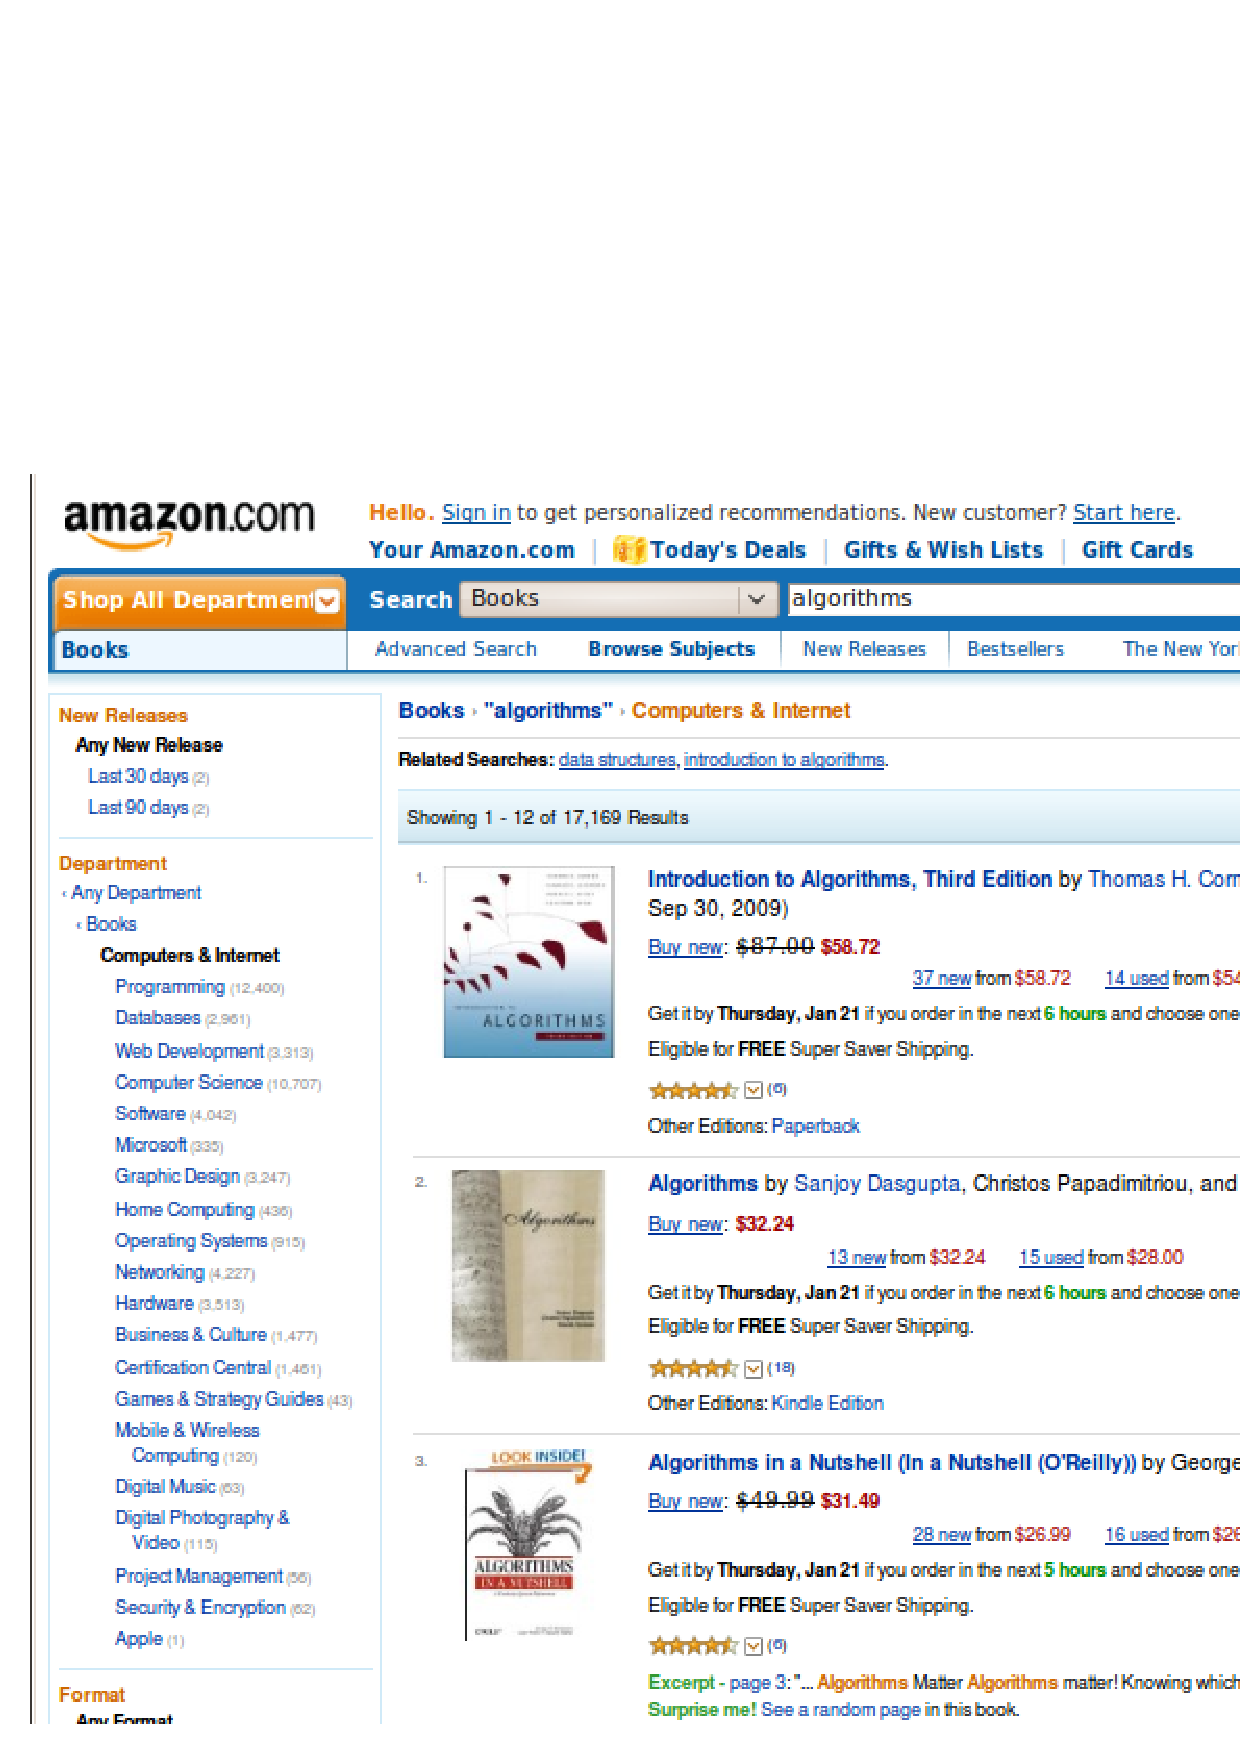
\includegraphics[scale=0.25]{img/ce}
\end{figure}

\newpage
    \item Motivação
    \begin{my_itemize}
    \item Extrair os itens de sites de comércio eletrônico
    \item Agregar informação a sites de busca de preço
    \end{my_itemize}

    \item {\color{yellow}Trabalhos Relacionados}

    \item {\color{yellow}Corpus}

  \end{my_itemize}
\end{frame}

\section{Andamento}
\begin{frame}
  \subsection{Ambiente de Experimentação}
  \frametitle{Ambiente de Experimentação}
\begin{center}
  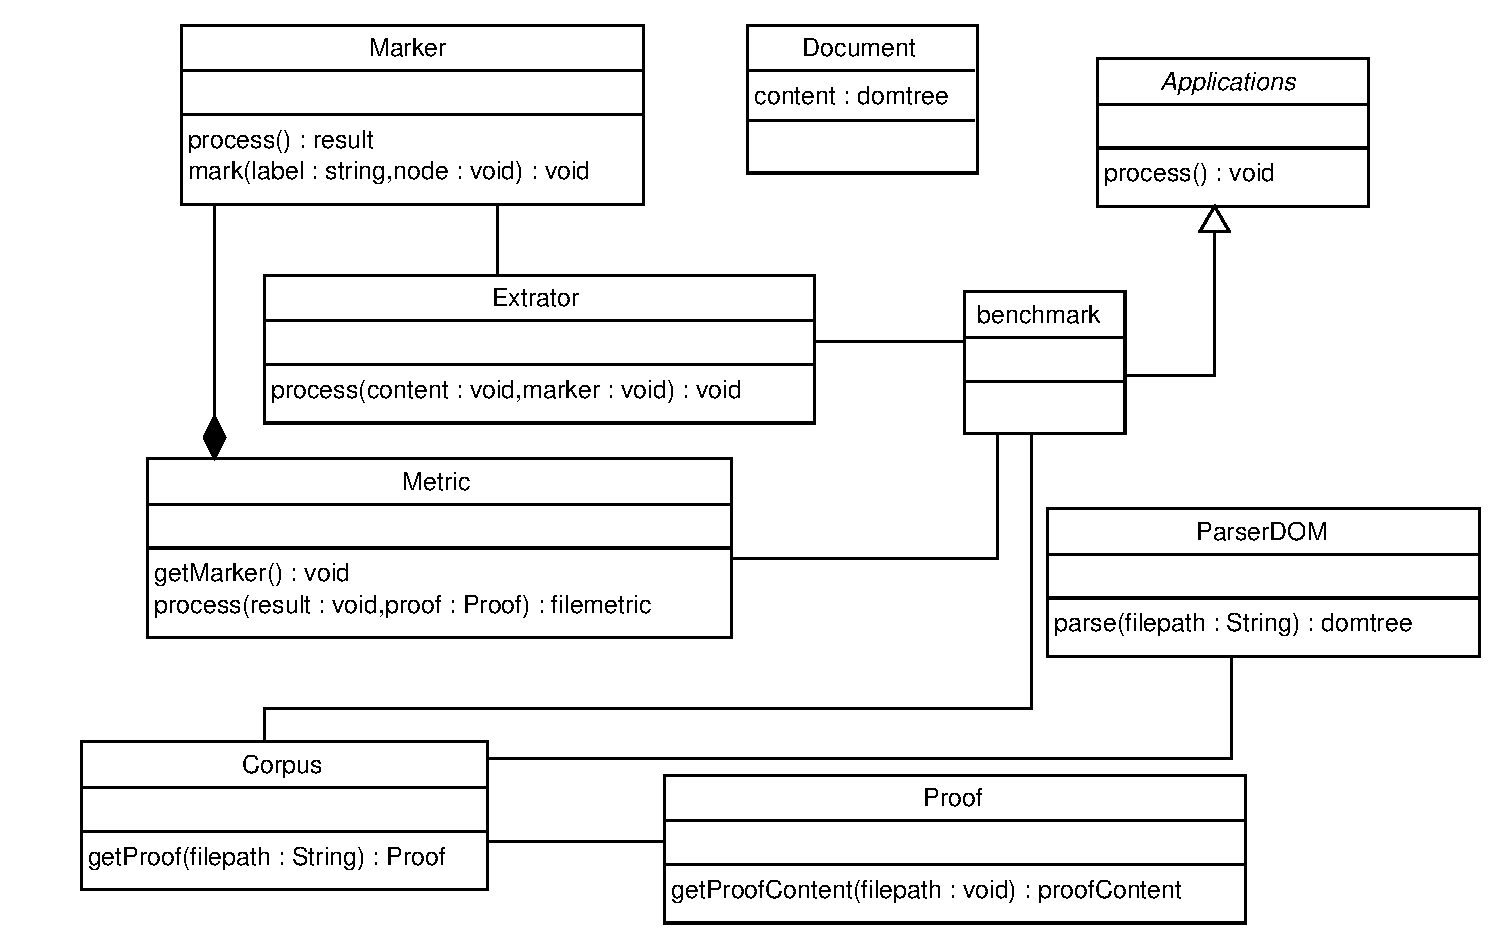
\includegraphics[width=1\textwidth]{img/classes}
\end{center}
\end{frame}

\begin{frame}
  \subsection{Andamento na identificação de tabela}
  \frametitle{Andamento na identificação de tabela}
  \begin{my_itemize}
   \item Dados estatísticos
   \begin{my_itemize}
   \item Número de tabelas (\textit{tag table}) em {\color{yellow}XX} documentos
   \item Número de tabelas genuínas em {\color{yellow}XX} documentos
   \end{my_itemize}

   \item Heurísticas existentes
   \begin{my_itemize}
   \item Regra básica: apenas verifica a semelhança entre os filhos no nó table
   \item Regra específica: Após aplicar a regra básica verifica se existem pelo menos duas colunas que contêm informação nessa tabela. Lista não são marcados como tabela.
   \end{my_itemize}
  \end{my_itemize}
\end{frame}

\begin{frame}
  \subsection{Cronograma}
  \frametitle{Cronograma}
  \begin{center}
  {\small
  \begin{tabular}{| c | p{8cm} |}
    \hline
    Mês & Tarefa \\ \hline

    Janeiro & Investigar e melhorar resultados para a tarefa de identificação de tabelas. \\ \hline

    Fevereiro & Coletar corpora para a tarefa de extração de itens e investigar heurísticas para resolução da tarefa \\ \hline

    Março & Avaliar resultados obtidos e buscar melhorar os resultados existentes na área \\ \hline

    Abril &  Melhorar os resultados obtidos e otimizar algoritmos para obter baixo custo computacional \\ \hline

    Maio & Verificar novos trabalhos na área e formalizar os resultados obtidos \\ \hline

    Junho & Escrever e apresentar dissertação \\ \hline

  \end{tabular}
}
  \end{center}

\end{frame}

%  \footnotetext[1]{Carteira pode ser definido como um conjunto de ativos.}

%  \begin{center}
%  \begin{tabular}{| c | c | c |}
%    \hline
%    Nome & Risco (Variância) & Retorno \\ \hline
%    BBAS4 & 0.000731 & 1.313531 \\ \hline
%    VALE5 & 0.000363 & 1.074398 \\ \hline
%    BBAS4 & 0.000731 & 1.313531 \\ \hline
%    VALE5 & 0.000363 & 1.074398 \\ \hline
%    PETR3 & 0.000215 & 1.275080 \\ \hline
%    USIM5 & 0.000693 & 1.123417 \\ \hline
%    PETR4 & 0.000208 & 1.250830 \\ \hline
%  \end{tabular}
%  \end{center}
%  \pause

%\begin{center}
%  \includegraphics[width=0.6\textwidth]{figuras/FroteiraEficiente}
%\end{center}

\section{Bibliografia}
\begin{frame}[allowframebreaks]
  \frametitle{Bibliografia}
   \bibliographystyle{abstract}
  \bibliography{proposta}
\end{frame}
\end{document}